\newpage

\section{Tipi di agenti}

4 tipi di agenti (dal meno generale a quello più generale):

\begin{itemize}
 \item simple reflex (reattivi)
 \item model-based reflex agents
 \item agenti basati su goal
 \item utility-based agent
\end{itemize}

Tutti questi possono essere trasformati in learning agents.\\

Notazione: di seguito con ``mondo'' si intende ``insieme di stati''. Gli schemi
dei seguenti agenti funzionano per incrementi (sono le parti in grassetto).

\subsection{Reflex agents}

Ambiente $\rightarrow$ Sensori $\rightarrow$ Capisco com'è il mondo in questo
istante $\rightarrow$ \textbf{Che azione dovrei fare? (dipende dalle regole
condizione/azione)} $\rightarrow$ Attuatori $\rightarrow$ Ambiente

\subsection{Model-based reflex agents}

Ambiente $\rightarrow$ Sensori $\rightarrow$ Capisco com'è il mondo in
questo istante \textbf{(come evolve e come influiscono su di esso le mie
azioni)} $\rightarrow$ Che azione dovrei fare? (dipende dalle regole
condizione/azione) $\rightarrow$ Attuatori $\rightarrow$ Ambiente

\subsection{Goal-based agents}

Ambiente $\rightarrow$ Sensori $\rightarrow$ Capisco com'è il mondo in questo
istante (come evolve e come influiscono su di esso le mie azioni) $\rightarrow$
\textbf{Come apparirebbe il mondo se eseguissi l'azione A? (ipotesi/test)}
$\rightarrow$ Che azione dovrei fare? (dipende dalle regole condizione/azione)
$\rightarrow$ Attuatori $\rightarrow$ Ambiente

\subsection{Utility-based agent}

Ambiente $\rightarrow$ Sensori $\rightarrow$ Capisco com'è il mondo in questo
istante (come evolve e come influiscono su di esso le mie azioni)
$\rightarrow$ Come apparirebbe il mondo se eseguissi l'azione A? (ipotesi/test)
$\rightarrow$ \textbf{Quanto soddisfatto sarei in questo stato?
(dipende dall'utilità)} $\rightarrow$ Che azione dovrei fare?
(dipende dalle regole condizione/azione) $\rightarrow$ Attuatori
$\rightarrow$ Ambiente

\subsection{Learning agents}

Sono agenti programmati in modo tale che apprendano, gestiscano e si adattino
ad ambienti sconosciuti.

Componenti di un learning agent:

\begin{itemize}
 \item Componente di \textbf{apprendimento}: per migliorare se stesso.
 \item \textbf{Performance} element: seleziona quali azioni compiere.
 \item \textbf{Critic} element: misura quanto ``bene'' l'agente si
comporta in relazione alla misura di performance.
 \item \textbf{Problem generation}: genera azioni con ``guadagno di
informazioni'' (suggerisce azioni sub-ottime che nel lungo
termine potrebbero rivelarsi migliori).
\end{itemize}

\subsection{Problem solving agents}

È un sottotipo degli agenti basati su obiettivo (goal-based agents).

Prima formula il \textbf{problema}, tramite un insieme di \textbf{stati}
(designandone uno iniziale), poi il \textbf{goal} (un insieme di stati
desiderabili in cui l'obiettivo è stato raggiunto) e un insieme di
\textbf{azioni}.
Infine specifica i \textbf{costi} di ricerca e di esecuzione. \\

\{Problema, insieme degli stati, goal, insieme delle azioni, costi
di ricerca ed esecuzione\}\\

Questo agente funziona in un ambiente \textit{statico, noto, osservabile e
deterministico}.

Un concetto importante è dato dal \textbf{modello di transizione}, che
descrive il risultato di una certa azione su un certo stato
(funzione ``successore'').

Un'azione che è possibile eseguire nello stato s si dice \textbf{applicabile}
in s.

La soluzione è data da un'appropriata \textbf{sequenza di azioni}.

Il processo di scoperta di una soluzione viene chiamato \textbf{ricerca}.

Lo spazio degli stati (diverso dall'insieme degli stati!) rappresenta
un'\textbf{astrazione} di un problema reale, che solitamente è molto complesso.

Un'astrazione è utile/valida se è possibile ``trasformare'' ogni soluzione
astratta in una soluzione nel mondo reale.

Un'astrazione dovrebbe essere ``più facile'' del problema che astrae.

\subsubsection{Esempio: formulazione di un problema}

Si consideri il problema dell'aspirapolvere. \\

\textbf{Insieme di stati}: 8 (sporco o pulito (4))*(destra o sinistra (2)).

\textbf{Insieme di azioni}: muoviti a destra, muoviti a sinistra, aspira.

\textbf{Goal}: arrivare agli stati (2) in cui non c'è sporco.

\textbf{Costo}: 1 unità per azione (è arbitrario in questo esempio).

\begin{figure}[H]
\centering
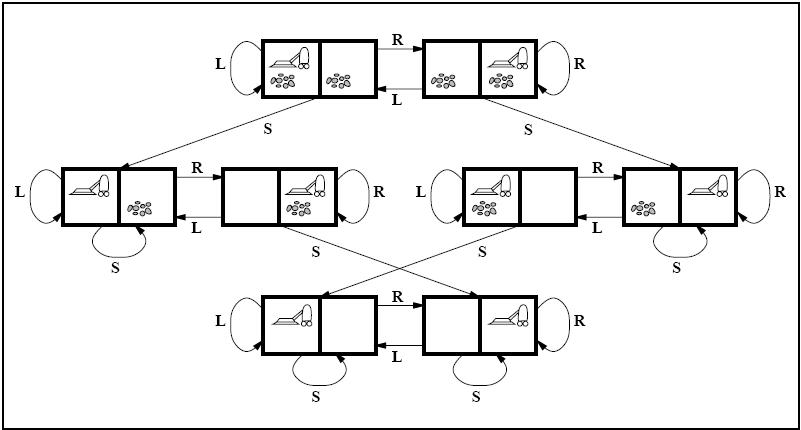
\includegraphics[width=0.7\textwidth]{vacuum.jpg}
\caption{grafo di transizione per il problema dell'aspirapolvere}
\label{fig:vacuum}
\end{figure}
